\section{Hyper Text Transfer Protocol}

Web pages are composed of multiple resources, including HTML documents, images, scripts, and other embedded elements. 
Each resource is uniquely identified by a Uniform Resource Locator (URL) or a Uniform Resource Identifier (URI), allowing clients to locate and access them over a network.
When a client requests a resource using a URL, the request is resolved through domain name resolution (DNS), followed by the retrieval of the requested data from the corresponding web server.

On the web, resources are managed by servers, identified through URIs, and accessed synchronously by clients using a request/response paradigm.
This model aligns with the Representational State Transfer (REST) architectural style, which enables scalable and stateless interactions between clients and servers.


\subsection{Communication}
HTTP follows a client-server architecture, where communication occurs as follows:
\begin{itemize}
    \item The client sends an HTTP request for a specific resource, identified by its URI.
    \item The server processes the request and responds with the requested resource or an appropriate status message.
\end{itemize}
HTTP is a stateless protocol, meaning each request is independent, and the server does not retain memory of previous interactions. 
This simplifies communication but requires additional mechanisms for maintaining user state when necessary.

HTTP requests are human-readable (ASCII-encoded) and follow a structured format. 
The request includes essential components such as the method, the target resource (URI), and optional headers containing metadata.
\begin{figure}[H]
    \centering
    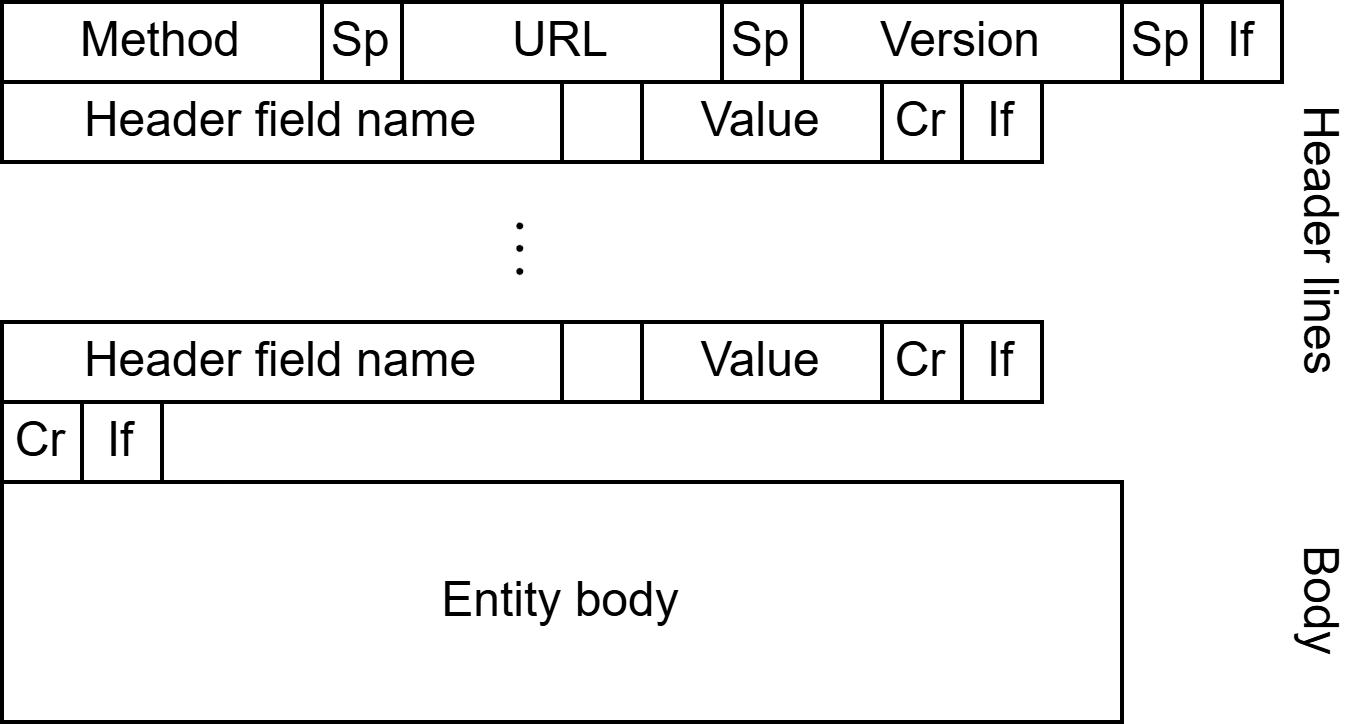
\includegraphics[width=0.5\linewidth]{images/http.png}
    \caption{HTTP request}
\end{figure}
HTTP responses follow a similar format, including a status code that indicates the outcome of the request:
\begin{itemize}
    \item \textit{Informational} (1xx): request received and processing continues.
    \item \textit{Success} (2xx): the request was successfully processed.
    \item \textit{Redirection} (3xx): further action is needed to complete the request.
    \item \textit{Client-side error} (4xx): the request contains incorrect syntax or cannot be fulfilled.
    \item \textit{Server-side error} (5xx): the server encountered an issue while processing the request.
\end{itemize}
\begin{figure}[H]
    \centering
    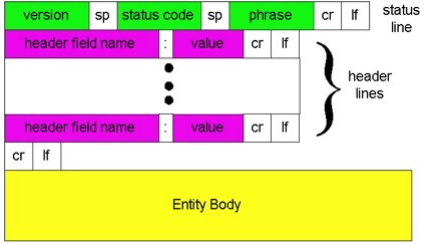
\includegraphics[width=0.5\linewidth]{images/http1.png}
    \caption{HTTP request}
\end{figure}